%!TEX root = ../Thesis.tex

%%%%%%%%%%%%%%%%%%%%%%%%%%%%%%%%%%%%%%%%%%%%%%%%%%%%%%%%%%%%%%%%%%%%%%%%
\chapter{Introduction}
%%%%%%%%%%%%%%%%%%%%%%%%%%%%%%%%%%%%%%%%%%%%%%%%%%%%%%%%%%%%%%%%%%%%%%%%

\begin{figure}[t]
  \centering
  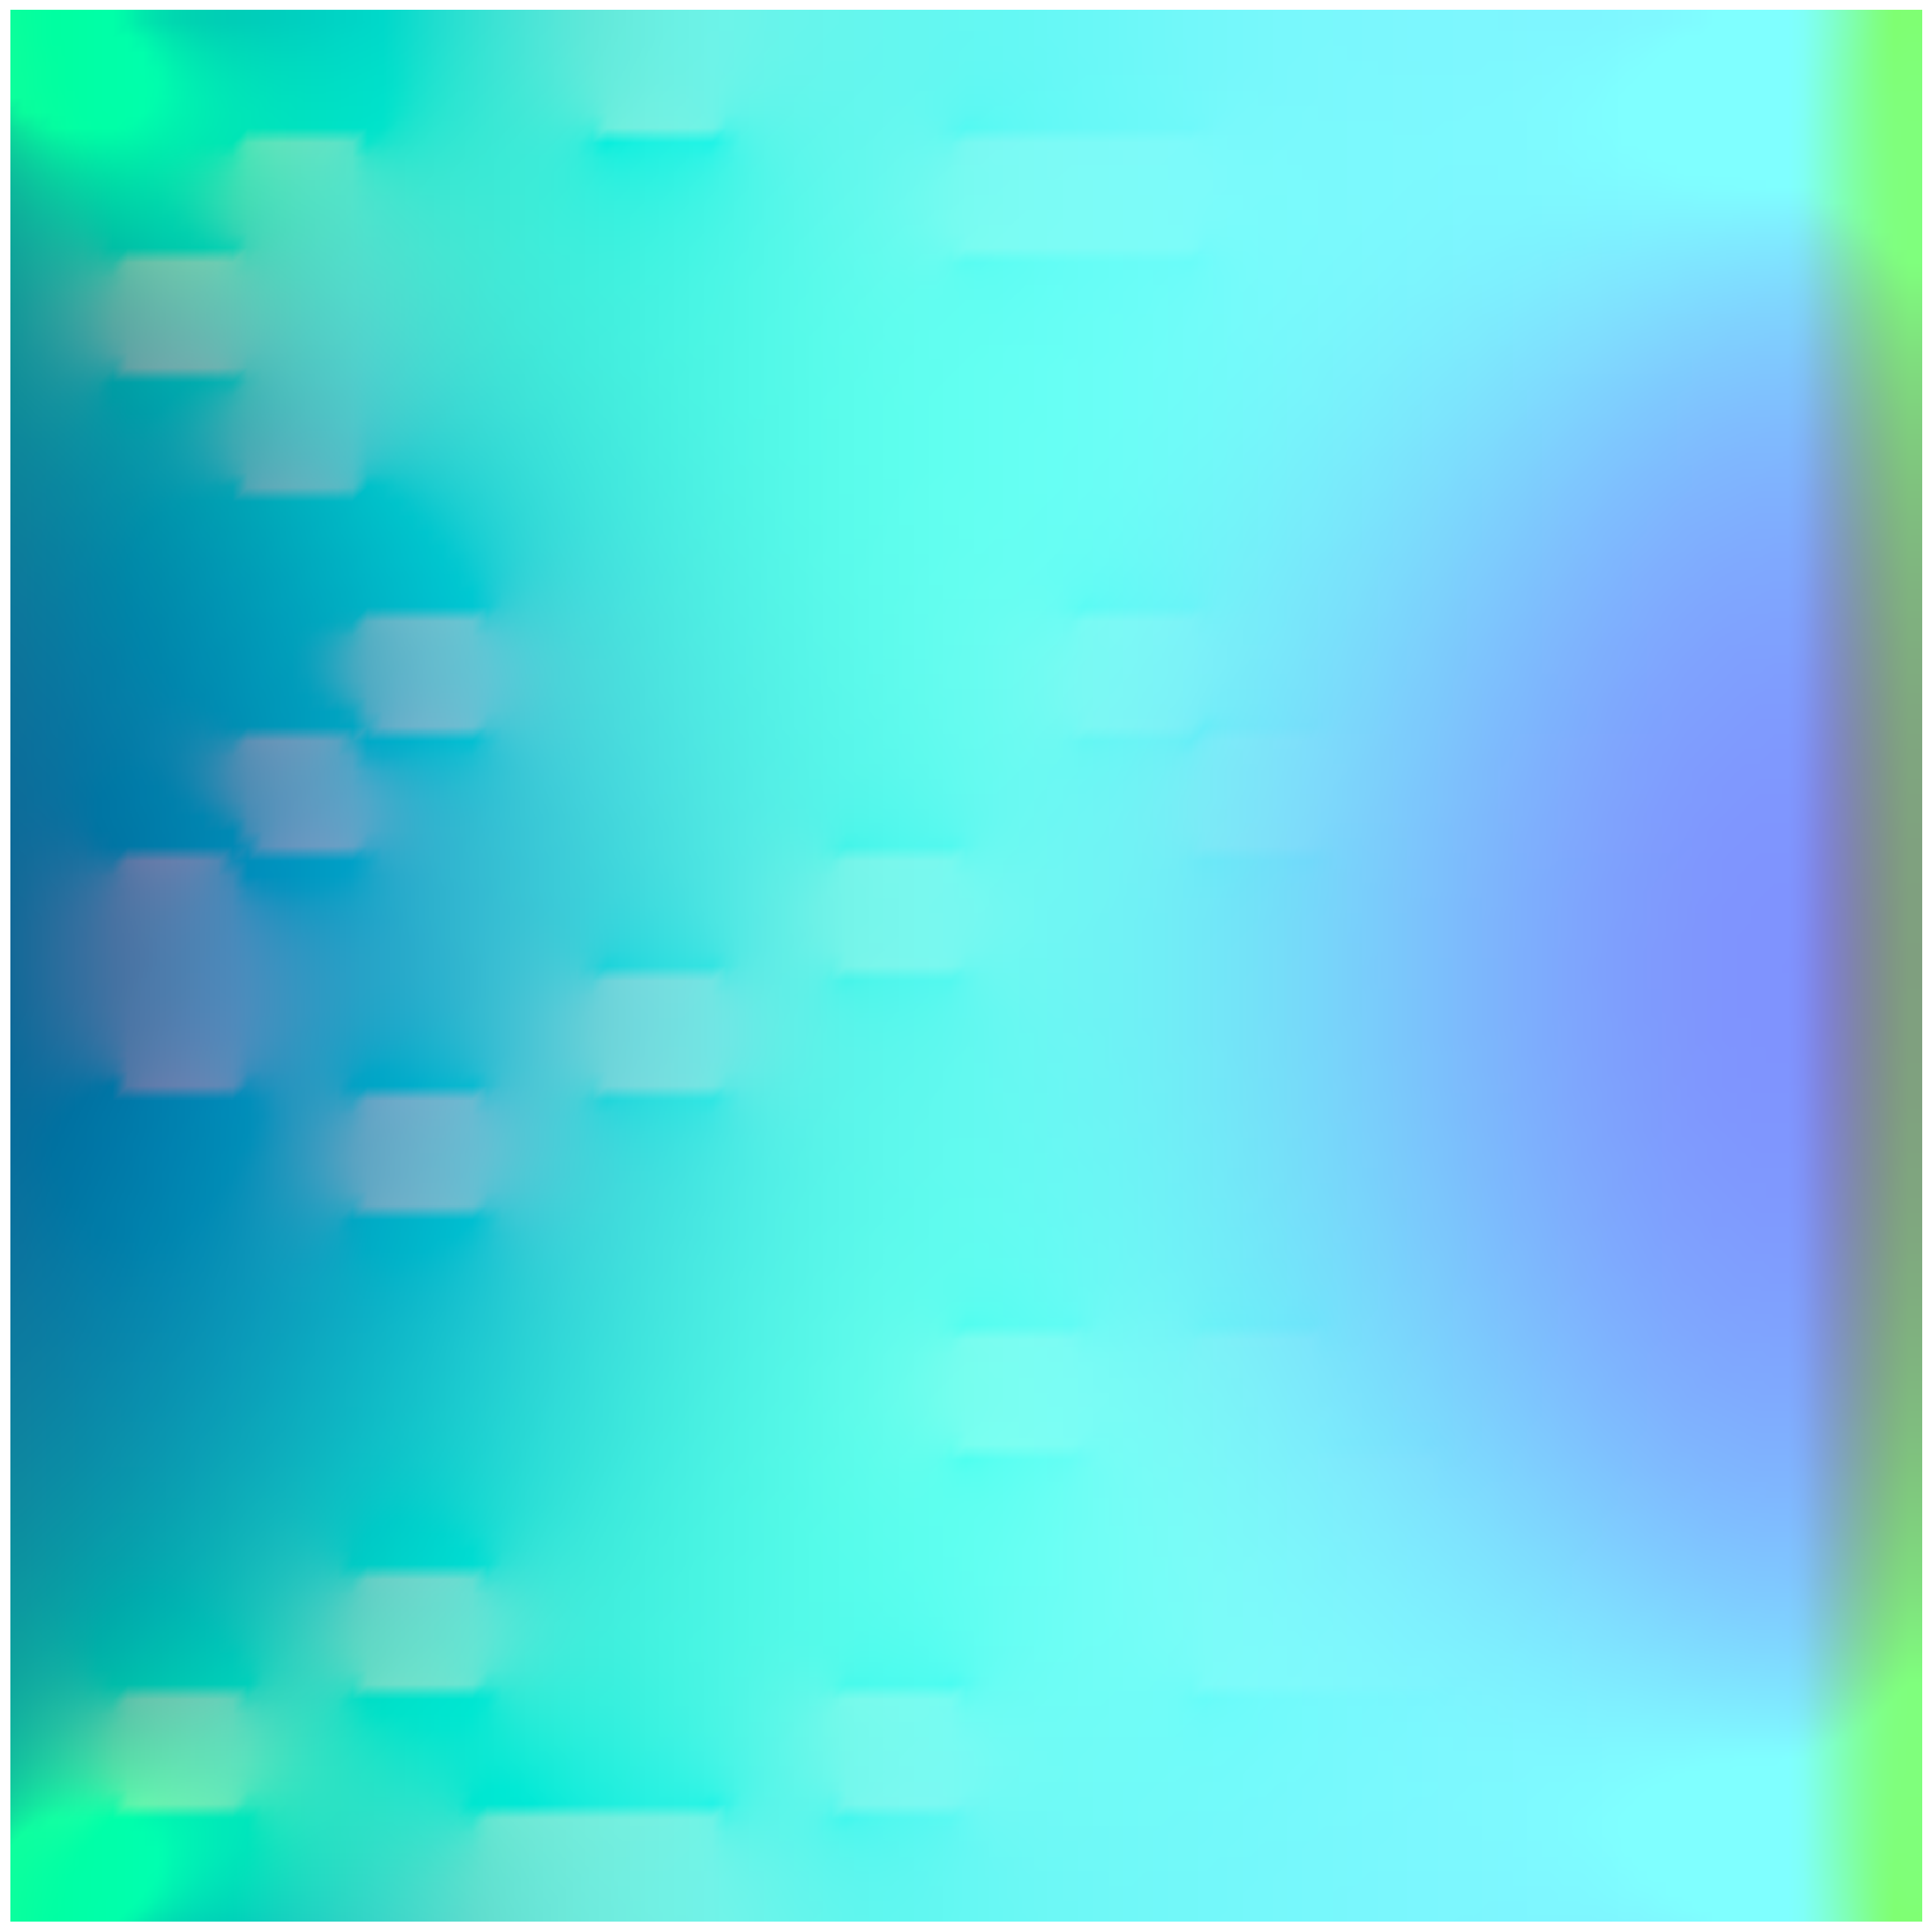
\includegraphics[width=0.5\linewidth]{figures/dummy}
  \caption{Do not state the obvious. Do not state the obvious. Do not state the obvious. Do not state the obvious. Do not state the obvious. Do not state the obvio.}
\end{figure}

Today data is often visualized as graphs to make it more readable and easier to understand and access. The problem with this is, that current research creates large datasets and the more data is visualized, the harder it gets to read the resulting graph. This predicament created the research ares of edge bundling techniques. These techniques allow graphs to become more readable and reveal patterns that were previously hidden.

